\documentclass[a4paper,portrait]{article}
%\documentclass[border=5mm, 12pt]{standalone}

%\usepackage[latin1]{inputenc}
\usepackage{graphicx}
\usepackage[margin=1.0cm]{geometry}
\usepackage{caption}
\usepackage{ulem}

\captionsetup{
   justification=raggedright,
   labelfont=bf,
   singlelinecheck=off
}

\renewcommand{\familydefault}{\sfdefault}
\renewcommand{\sfdefault}{phv}

\setcounter{figure}{3} % Set figure counter to one minus actual figure number

\begin{document}

\begin{figure}[!htbp]%[H]
%\begin{figure}[ht]
\centering
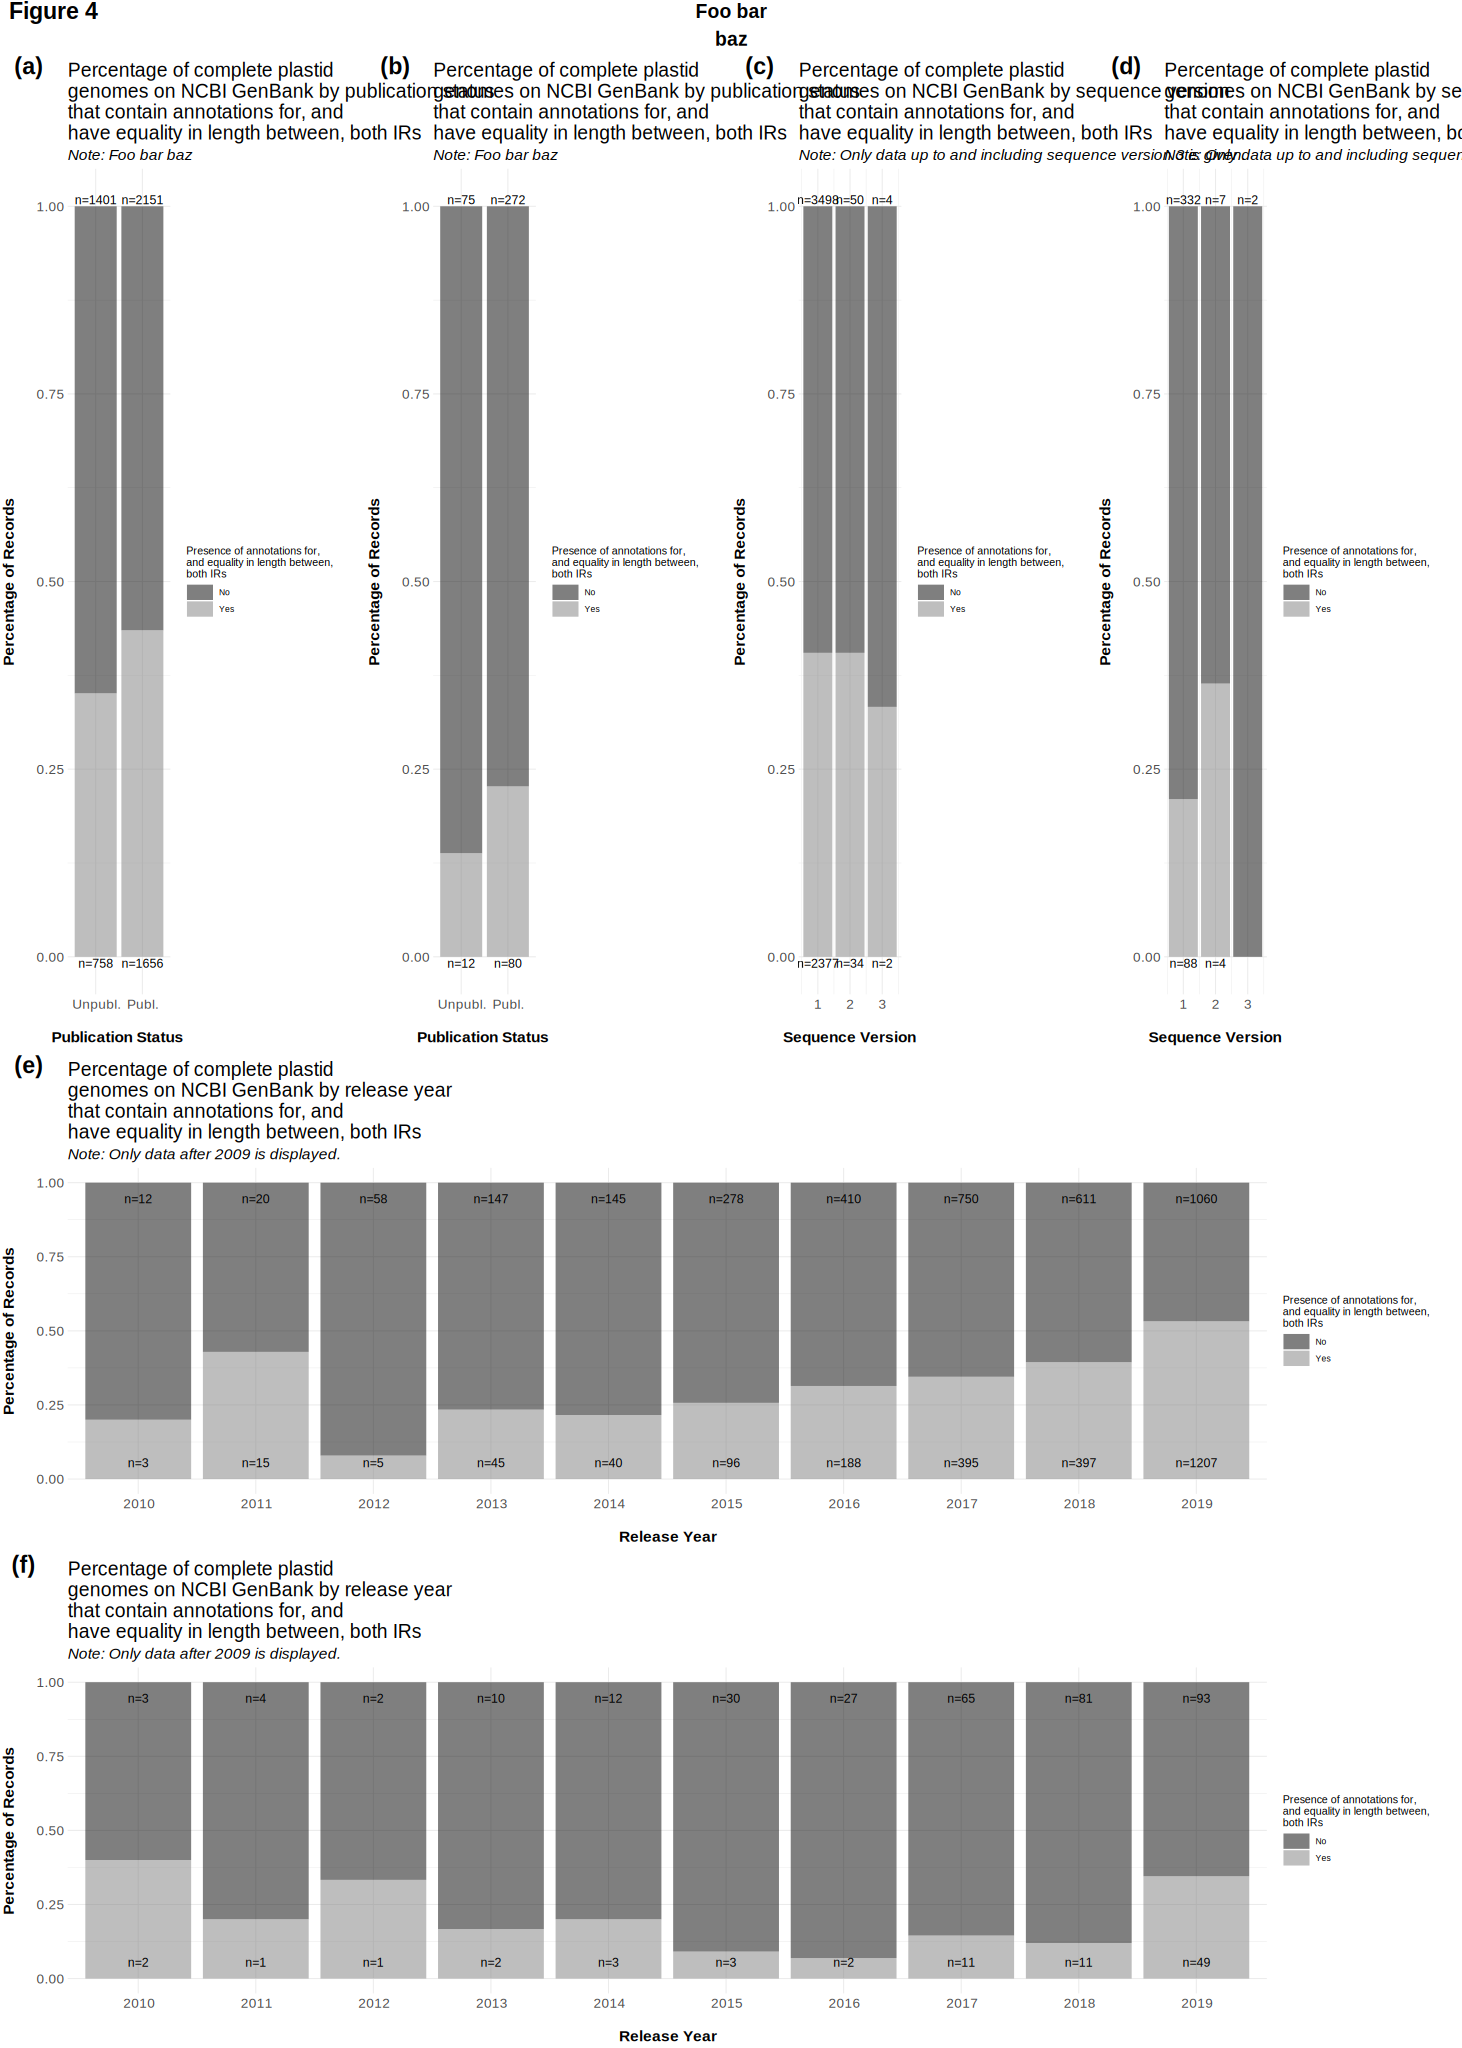
\includegraphics[width=1.00\linewidth]{input/MANUSCRIPT_Figure4.pdf}
\caption{Overview of the \sout{presence and length equality of IR annotations among all complete plastid genomes on GenBank. The plots of the upper row visualize the cumulative number of complete plastid genomes over the past 20 years that contain (light grey) or lack (dark grey) annotations for the IRs, separated by \textbf{(a)} angiosperms and \textbf{(b)} non-angiosperms. The plots in the center row visualize the cumulative number of complete plastid genomes over the past 20 years whose reported IR annotations display unequal lengths, separated by \textbf{(c)} angiosperms and \textbf{(d)} non-angiosperms. The plots in the bottom row visualize the distribution of length differences between the IRs of each plastid genome with unequal IR lengths, separated by \textbf{(e)} angiosperms and \textbf{(f)} non-angiosperms. The x-axis of the plots in the bottom row is set to a logarithmic scale.} All duplicate records generated via the NCBI RefSeq database were excluded prior to plotting.}

\label{fig:Figure4}
\end{figure}

\end{document}
